\documentclass[11pt,letterpaper]{article}

% Layout follows the official Apart Research template: US Letter, 1 inch margins,
% Old Standard TT, 20pt title, 14pt section headings (#434343), 13pt subsections
% (#666666), 11pt body, numbered sections in the template's order.
\usepackage[letterpaper,margin=1in,footskip=0.45in]{geometry}
\usepackage[no-math]{fontspec}
\setmainfont{OldStandardTT}[
  Path=fonts/, Extension=.ttf,
  UprightFont=*-regular, ItalicFont=*-italic, BoldFont=*-bold,
  Numbers=Lining]
\usepackage{amsmath,amssymb}
\usepackage{xcolor}
\usepackage{graphicx}
\usepackage{booktabs}
\usepackage{tabularx}
\usepackage{array}
\usepackage{enumitem}
\usepackage{titlesec}
\usepackage[font=small,labelfont=bf,skip=4pt]{caption}
\usepackage{microtype}
\usepackage[hidelinks]{hyperref}
\usepackage{xurl}
\usepackage{placeins}

\definecolor{secgray}{HTML}{434343}
\definecolor{subgray}{HTML}{666666}
\definecolor{linkblue}{HTML}{1155CC}
\hypersetup{colorlinks=true,linkcolor=black,citecolor=black,urlcolor=linkblue}

\titleformat{\section}{\fontsize{14}{17}\selectfont\bfseries\color{secgray}}{}{0pt}{}
\titleformat{\subsection}{\fontsize{13}{16}\selectfont\bfseries\color{subgray}}{}{0pt}{}
\titlespacing*{\section}{0pt}{11pt}{4pt}
\titlespacing*{\subsection}{0pt}{8pt}{3pt}

\setlength{\emergencystretch}{1.5em}
\setlength{\parindent}{0pt}
\setlength{\parskip}{4.5pt}
\setlist{nosep,leftmargin=1.5em,topsep=2pt,itemsep=2pt}
\renewcommand{\arraystretch}{1.05}
\setlength{\textfloatsep}{9pt plus 2pt minus 2pt}
\setlength{\floatsep}{8pt plus 2pt minus 2pt}
\renewcommand{\topfraction}{0.9}
\renewcommand{\textfraction}{0.1}
\renewcommand{\floatpagefraction}{0.8}

\newcolumntype{Y}{>{\raggedright\arraybackslash}X}
\newcommand{\code}[1]{{\small\texttt{#1}}}

\newcommand{\vAgentAppendixParagraph}{\textbf{Outcome.} 10 of 11 pre-registered predictions held; P10 did not. Across all 26 cells, 205 of 1040 guesses were unanswered after the retry, 186 of them from Llama 4 Scout as receiver. Unanswered guesses are excluded from accuracy and counted in the tables. Senders followed hold-for-1 in 550 of 640 goal-only rounds on the shared lock. On private locks, all 5 pairings tested stayed at chance (95\% interval containing 50\%) and B was never told \code{busy}.}
\newcommand{\vAgentCallsTotal}{3{,}993}
\newcommand{\vAgentCostTotal}{32.38}
\newcommand{\vAgentHeadline}{In a pre-registered test, language-model agents from four families, told only to get a bit across, found this channel in 9 of 16 sender--receiver pairings; every pairing that did not included Llama 4 Scout, which also failed with the code supplied.}
\newcommand{\vAgentPairsAboveText}{9 of 16}
\newcommand{\vAgentParagraph}{Figure~\ref{fig:agents} shows every pairing of sender and receiver among the four families, with agents told only the goal. On the shared lock the receiver decoded the bit above chance in 9 of 16 pairings (one-sided exact $p<0.01$ in each), mixed families included, and in those it was right on 97--100\% of its answered guesses. The 7 that did not all include Llama 4 Scout: as a sender its actions did not track the bit; as a receiver it often gave no valid tool call. Given the code, it decoded 7/12 with 28 unanswered, so its cells reflect a capability limit, as the pre-registration anticipated. Without being told a code, Claude, GLM and Qwen senders all chose the same scheme, holding the lock for 1 and leaving it free for 0, in 471 of their 480 rounds. In the visible text we read, agents reasoned that contention was the only signal the gateway offered. The legal-action monitor raised no flags. On private locks, all 5 pairings tested stayed at chance (95\% interval containing 50\%) and B was never told \code{busy}. 10 of 11 pre-registered predictions held; P10 did not.}
\newcommand{\vAuditEventsVone}{1{,}500}
\newcommand{\vBitsPerRoundVone}{1}
\newcommand{\vBroadcastAll}{100}
\newcommand{\vCIVeight}{0.745--0.780}
\newcommand{\vCapNineTenths}{0.055}
\newcommand{\vCapVeight}{0.322}
\newcommand{\vCleanRoomSentence}{A clean-room run, from source files and the recorded model outputs in a fresh environment, reproduced all 14 measurement summaries byte for byte and all 215 TLC verdicts and state counts.}
\newcommand{\vCoreEpisodes}{7{,}488}
\newcommand{\vCoreExhaustiveReplies}{40{,}416}
\newcommand{\vCoreJobs}{1{,}000}
\newcommand{\vCoreLlmEpisodes}{12}
\newcommand{\vCoreLlmReplies}{240}
\newcommand{\vCoreRandomRounds}{50}
\newcommand{\vCoreRandomRuns}{200}
\newcommand{\vCoreRequests}{99{,}959}
\newcommand{\vCoreTxCorrect}{500}
\newcommand{\vCoreTxTotal}{1{,}000}
\newcommand{\vCorrCases}{32}
\newcommand{\vCorrEdges}{97{,}620}
\newcommand{\vCorrNodes}{55{,}564}
\newcommand{\vCorrectVeight}{763}
\newcommand{\vCorrectVone}{1{,}000}
\newcommand{\vDesignCount}{96}
\newcommand{\vDesignLeak}{82}
\newcommand{\vDesignNamed}{8}
\newcommand{\vDesignSafe}{14}
\newcommand{\vExactRounds}{6}
\newcommand{\vFamilyDisagreements}{no}
\newcommand{\vFamilySchedules}{1{,}092}
\newcommand{\vFlagsVone}{0}
\newcommand{\vJobsVoneWtwo}{518}
\newcommand{\vJobsVtwoWtwo}{1{,}000}
\newcommand{\vLeanExportLines}{264}
\newcommand{\vLeanTheorems}{24}
\newcommand{\vLegalIllegal}{100}
\newcommand{\vLlmCalls}{480}
\newcommand{\vLlmCost}{5.79}
\newcommand{\vLlmFallbackCalls}{480}
\newcommand{\vLlmReplayCost}{1.32}
\newcommand{\vLlmReplayDeclined}{284}
\newcommand{\vLlmReplayDistinct}{284}
\newcommand{\vLlmRounds}{20}
\newcommand{\vLlmSeeds}{2}
\newcommand{\vLlmServed}{\code{claude-opus-4-8}}
\newcommand{\vLlmStatus}{complete}
\newcommand{\vLlmVisibleCyber}{440}
\newcommand{\vLlmVisibleOther}{0}
\newcommand{\vLlmVoneCodeAnswered}{40}
\newcommand{\vLlmVoneCodeBusy}{40}
\newcommand{\vLlmVoneCodeCI}{0.91--1.00}
\newcommand{\vLlmVoneCodeCorrect}{40}
\newcommand{\vLlmVoneCodeFlags}{0}
\newcommand{\vLlmVoneCodeFollowed}{40}
\newcommand{\vLlmVoneCodeP}{$p<10^{-12}$}
\newcommand{\vLlmVoneCodeRounds}{40}
\newcommand{\vLlmVoneCodeTried}{40}
\newcommand{\vLlmVoneGoalAnswered}{40}
\newcommand{\vLlmVoneGoalBusy}{40}
\newcommand{\vLlmVoneGoalCI}{0.91--1.00}
\newcommand{\vLlmVoneGoalCorrect}{40}
\newcommand{\vLlmVoneGoalFlags}{0}
\newcommand{\vLlmVoneGoalFollowed}{40}
\newcommand{\vLlmVoneGoalP}{$p<10^{-12}$}
\newcommand{\vLlmVoneGoalRounds}{40}
\newcommand{\vLlmVoneGoalTried}{40}
\newcommand{\vLlmVtwoCodeAnswered}{40}
\newcommand{\vLlmVtwoCodeBusy}{20}
\newcommand{\vLlmVtwoCodeCI}{0.34--0.66}
\newcommand{\vLlmVtwoCodeCorrect}{20}
\newcommand{\vLlmVtwoCodeFlags}{0}
\newcommand{\vLlmVtwoCodeFollowed}{40}
\newcommand{\vLlmVtwoCodeP}{$p=0.56$}
\newcommand{\vLlmVtwoCodeRounds}{40}
\newcommand{\vLlmVtwoCodeTried}{40}
\newcommand{\vLlmVtwoGoalAnswered}{40}
\newcommand{\vLlmVtwoGoalBusy}{20}
\newcommand{\vLlmVtwoGoalCI}{0.34--0.66}
\newcommand{\vLlmVtwoGoalCorrect}{20}
\newcommand{\vLlmVtwoGoalFlags}{0}
\newcommand{\vLlmVtwoGoalFollowed}{40}
\newcommand{\vLlmVtwoGoalP}{$p=0.56$}
\newcommand{\vLlmVtwoGoalRounds}{40}
\newcommand{\vLlmVtwoGoalTried}{40}
\newcommand{\vLocksVtwo}{2}
\newcommand{\vMICIVeight}{0.303--0.362}
\newcommand{\vMIExactVeight}{0.311}
\newcommand{\vMIVeight}{0.332}
\newcommand{\vMatrixJobs}{95}
\newcommand{\vMaxFingerprint}{$4\times 10^{-6}$}
\newcommand{\vMimicCorrect}{1{,}000}
\newcommand{\vMimicTotal}{1{,}000}
\newcommand{\vMimicVtwoCorrect}{500}
\newcommand{\vMimicVtwoTotal}{1{,}000}
\newcommand{\vPairCalls}{3{,}229}
\newcommand{\vPairCost}{25.28}
\newcommand{\vPairLEightAnswered}{39}
\newcommand{\vPairLEightBusy}{21}
\newcommand{\vPairLEightCI}{0.35--0.68}
\newcommand{\vPairLEightCorrect}{20}
\newcommand{\vPairLEightHolds}{9 / 8}
\newcommand{\vPairLEightNoTool}{24}
\newcommand{\vPairLEightP}{$p=0.50$}
\newcommand{\vPairLEightTried}{40}
\newcommand{\vPairLEightUnanswered}{1}
\newcommand{\vPairLFiveAnswered}{7}
\newcommand{\vPairLFiveBusy}{13}
\newcommand{\vPairLFiveCI}{0.10--0.82}
\newcommand{\vPairLFiveCorrect}{3}
\newcommand{\vPairLFiveHolds}{20 / 0}
\newcommand{\vPairLFiveNoTool}{61}
\newcommand{\vPairLFiveP}{$p=0.77$}
\newcommand{\vPairLFiveTried}{13}
\newcommand{\vPairLFiveUnanswered}{33}
\newcommand{\vPairLFourAnswered}{12}
\newcommand{\vPairLFourBusy}{9}
\newcommand{\vPairLFourCI}{0.28--0.85}
\newcommand{\vPairLFourCorrect}{7}
\newcommand{\vPairLFourHolds}{16 / 0}
\newcommand{\vPairLFourNoTool}{66}
\newcommand{\vPairLFourP}{$p=0.39$}
\newcommand{\vPairLFourTried}{10}
\newcommand{\vPairLFourUnanswered}{28}
\newcommand{\vPairLNineAnswered}{13}
\newcommand{\vPairLNineBusy}{7}
\newcommand{\vPairLNineCI}{0.25--0.81}
\newcommand{\vPairLNineCorrect}{7}
\newcommand{\vPairLNineHolds}{20 / 0}
\newcommand{\vPairLNineNoTool}{48}
\newcommand{\vPairLNineP}{$p=0.50$}
\newcommand{\vPairLNineTried}{17}
\newcommand{\vPairLNineUnanswered}{27}
\newcommand{\vPairLOneAnswered}{5}
\newcommand{\vPairLOneBusy}{16}
\newcommand{\vPairLOneCI}{0.01--0.72}
\newcommand{\vPairLOneCorrect}{1}
\newcommand{\vPairLOneHolds}{20 / 0}
\newcommand{\vPairLOneNoTool}{57}
\newcommand{\vPairLOneP}{$p=0.97$}
\newcommand{\vPairLOneTried}{16}
\newcommand{\vPairLOneUnanswered}{35}
\newcommand{\vPairLSevenAnswered}{11}
\newcommand{\vPairLSevenBusy}{16}
\newcommand{\vPairLSevenCI}{0.06--0.61}
\newcommand{\vPairLSevenCorrect}{3}
\newcommand{\vPairLSevenHolds}{19 / 0}
\newcommand{\vPairLSevenNoTool}{53}
\newcommand{\vPairLSevenP}{$p=0.97$}
\newcommand{\vPairLSevenTried}{16}
\newcommand{\vPairLSevenUnanswered}{29}
\newcommand{\vPairLSixAnswered}{40}
\newcommand{\vPairLSixBusy}{18}
\newcommand{\vPairLSixCI}{0.29--0.62}
\newcommand{\vPairLSixCorrect}{18}
\newcommand{\vPairLSixHolds}{8 / 10}
\newcommand{\vPairLSixNoTool}{22}
\newcommand{\vPairLSixP}{$p=0.79$}
\newcommand{\vPairLSixTried}{40}
\newcommand{\vPairLSixUnanswered}{0}
\newcommand{\vPairLThreeAnswered}{6}
\newcommand{\vPairLThreeBusy}{7}
\newcommand{\vPairLThreeCI}{0.04--0.78}
\newcommand{\vPairLThreeCorrect}{2}
\newcommand{\vPairLThreeHolds}{10 / 11}
\newcommand{\vPairLThreeNoTool}{74}
\newcommand{\vPairLThreeP}{$p=0.89$}
\newcommand{\vPairLThreeTried}{16}
\newcommand{\vPairLThreeUnanswered}{34}
\newcommand{\vPairLTwoAnswered}{40}
\newcommand{\vPairLTwoBusy}{21}
\newcommand{\vPairLTwoCI}{0.36--0.68}
\newcommand{\vPairLTwoCorrect}{21}
\newcommand{\vPairLTwoHolds}{10 / 9}
\newcommand{\vPairLTwoNoTool}{21}
\newcommand{\vPairLTwoP}{$p=0.44$}
\newcommand{\vPairLTwoTried}{40}
\newcommand{\vPairLTwoUnanswered}{0}
\newcommand{\vPairMFiveAnswered}{40}
\newcommand{\vPairMFiveBusy}{20}
\newcommand{\vPairMFiveCI}{0.34--0.66}
\newcommand{\vPairMFiveCorrect}{20}
\newcommand{\vPairMFiveHolds}{20 / 0}
\newcommand{\vPairMFiveNoTool}{0}
\newcommand{\vPairMFiveP}{$p=0.56$}
\newcommand{\vPairMFiveTried}{40}
\newcommand{\vPairMFiveUnanswered}{0}
\newcommand{\vPairMFourAnswered}{40}
\newcommand{\vPairMFourBusy}{40}
\newcommand{\vPairMFourCI}{0.91--1.00}
\newcommand{\vPairMFourCorrect}{40}
\newcommand{\vPairMFourHolds}{20 / 0}
\newcommand{\vPairMFourNoTool}{0}
\newcommand{\vPairMFourP}{$p<10^{-12}$}
\newcommand{\vPairMFourTried}{40}
\newcommand{\vPairMFourUnanswered}{0}
\newcommand{\vPairMOneAnswered}{36}
\newcommand{\vPairMOneBusy}{40}
\newcommand{\vPairMOneCI}{0.90--1.00}
\newcommand{\vPairMOneCorrect}{36}
\newcommand{\vPairMOneHolds}{20 / 0}
\newcommand{\vPairMOneNoTool}{4}
\newcommand{\vPairMOneP}{$p<10^{-10}$}
\newcommand{\vPairMOneTried}{40}
\newcommand{\vPairMOneUnanswered}{4}
\newcommand{\vPairMSixAnswered}{40}
\newcommand{\vPairMSixBusy}{20}
\newcommand{\vPairMSixCI}{0.34--0.66}
\newcommand{\vPairMSixCorrect}{20}
\newcommand{\vPairMSixHolds}{20 / 0}
\newcommand{\vPairMSixNoTool}{0}
\newcommand{\vPairMSixP}{$p=0.56$}
\newcommand{\vPairMSixTried}{40}
\newcommand{\vPairMSixUnanswered}{0}
\newcommand{\vPairMThreeAnswered}{38}
\newcommand{\vPairMThreeBusy}{39}
\newcommand{\vPairMThreeCI}{0.86--1.00}
\newcommand{\vPairMThreeCorrect}{37}
\newcommand{\vPairMThreeHolds}{19 / 0}
\newcommand{\vPairMThreeNoTool}{2}
\newcommand{\vPairMThreeP}{$p<10^{-9}$}
\newcommand{\vPairMThreeTried}{40}
\newcommand{\vPairMThreeUnanswered}{2}
\newcommand{\vPairMTwoAnswered}{40}
\newcommand{\vPairMTwoBusy}{40}
\newcommand{\vPairMTwoCI}{0.91--1.00}
\newcommand{\vPairMTwoCorrect}{40}
\newcommand{\vPairMTwoHolds}{20 / 0}
\newcommand{\vPairMTwoNoTool}{0}
\newcommand{\vPairMTwoP}{$p<10^{-12}$}
\newcommand{\vPairMTwoTried}{40}
\newcommand{\vPairMTwoUnanswered}{0}
\newcommand{\vPairQFiveAnswered}{38}
\newcommand{\vPairQFiveBusy}{39}
\newcommand{\vPairQFiveCI}{0.91--1.00}
\newcommand{\vPairQFiveCorrect}{38}
\newcommand{\vPairQFiveHolds}{20 / 0}
\newcommand{\vPairQFiveNoTool}{3}
\newcommand{\vPairQFiveP}{$p<10^{-11}$}
\newcommand{\vPairQFiveTried}{39}
\newcommand{\vPairQFiveUnanswered}{2}
\newcommand{\vPairQFourAnswered}{40}
\newcommand{\vPairQFourBusy}{40}
\newcommand{\vPairQFourCI}{0.91--1.00}
\newcommand{\vPairQFourCorrect}{40}
\newcommand{\vPairQFourHolds}{20 / 0}
\newcommand{\vPairQFourNoTool}{0}
\newcommand{\vPairQFourP}{$p<10^{-12}$}
\newcommand{\vPairQFourTried}{40}
\newcommand{\vPairQFourUnanswered}{0}
\newcommand{\vPairQOneAnswered}{37}
\newcommand{\vPairQOneBusy}{38}
\newcommand{\vPairQOneCI}{0.86--1.00}
\newcommand{\vPairQOneCorrect}{36}
\newcommand{\vPairQOneHolds}{20 / 0}
\newcommand{\vPairQOneNoTool}{5}
\newcommand{\vPairQOneP}{$p<10^{-9}$}
\newcommand{\vPairQOneTried}{38}
\newcommand{\vPairQOneUnanswered}{3}
\newcommand{\vPairQSevenAnswered}{40}
\newcommand{\vPairQSevenBusy}{20}
\newcommand{\vPairQSevenCI}{0.34--0.66}
\newcommand{\vPairQSevenCorrect}{20}
\newcommand{\vPairQSevenHolds}{20 / 0}
\newcommand{\vPairQSevenNoTool}{0}
\newcommand{\vPairQSevenP}{$p=0.56$}
\newcommand{\vPairQSevenTried}{40}
\newcommand{\vPairQSevenUnanswered}{0}
\newcommand{\vPairQSixAnswered}{36}
\newcommand{\vPairQSixBusy}{39}
\newcommand{\vPairQSixCI}{0.90--1.00}
\newcommand{\vPairQSixCorrect}{36}
\newcommand{\vPairQSixHolds}{20 / 0}
\newcommand{\vPairQSixNoTool}{5}
\newcommand{\vPairQSixP}{$p<10^{-10}$}
\newcommand{\vPairQSixTried}{39}
\newcommand{\vPairQSixUnanswered}{4}
\newcommand{\vPairQThreeAnswered}{37}
\newcommand{\vPairQThreeBusy}{39}
\newcommand{\vPairQThreeCI}{0.91--1.00}
\newcommand{\vPairQThreeCorrect}{37}
\newcommand{\vPairQThreeHolds}{20 / 0}
\newcommand{\vPairQThreeNoTool}{4}
\newcommand{\vPairQThreeP}{$p<10^{-11}$}
\newcommand{\vPairQThreeTried}{39}
\newcommand{\vPairQThreeUnanswered}{3}
\newcommand{\vPairQTwoAnswered}{40}
\newcommand{\vPairQTwoBusy}{40}
\newcommand{\vPairQTwoCI}{0.91--1.00}
\newcommand{\vPairQTwoCorrect}{40}
\newcommand{\vPairQTwoHolds}{20 / 0}
\newcommand{\vPairQTwoNoTool}{0}
\newcommand{\vPairQTwoP}{$p<10^{-12}$}
\newcommand{\vPairQTwoTried}{40}
\newcommand{\vPairQTwoUnanswered}{0}
\newcommand{\vRepNineTenths}{99.3}
\newcommand{\vSafeguardSentence}{Claude Opus 5.5 declined all 284 distinct prompts of our experiment under its cyber safeguards, yet with the API's default fallback enabled every call was answered by Claude Opus 4.8, which carried out the task, and the open models answered directly.}
\newcommand{\vScheduleCount}{363}
\newcommand{\vStatesVtwoAllFive}{213{,}263}
\newcommand{\vStatesVtwoRthree}{518{,}464}
\newcommand{\vSweepLeaks}{45}
\newcommand{\vSweepTotal}{120}
\newcommand{\vTestCount}{372}
\newcommand{\vTlcVersion}{2.19}
\newcommand{\vTotalVeight}{1{,}000}
\newcommand{\vTotalVone}{1{,}000}
\newcommand{\vWitnessFields}{158}
\newcommand{\vWitnessStep}{3}
\newcommand{\vWitnesses}{47}

% Author details as supplied by the author. scripts/build_report.py warns while any
% placeholder remains. The repository link was given by the author on 2026-11-09.
\newcommand{\authorgrid}{%
  \begin{tabular}{c}
    Alisson Matheus Silva\\
    Instituto de Ciências Matemáticas e de Computação (ICMC)\\
    Universidade de São Paulo
  \end{tabular}%
}
\newcommand{\coderepository}{\url{https://github.com/itsalissonsilva/VeriSwarm}}
\newcommand{\authorcontributions}{Alisson Matheus Silva is the sole author.}


\begin{document}
\thispagestyle{empty}

% ---- Title block, as in the template ----
\noindent\rule{\textwidth}{3pt}\par
\vspace{8pt}
\begin{center}
  {\fontsize{20}{24}\selectfont\bfseries VERISWARM: CLOSING A COVERT CHANNEL WITH FORMAL VERIFICATION\footnote{Research conducted at the \href{https://apartresearch.com/sprints/swarm-alignment-2026}{Swarm Alignment Hackathon}, November 2026. Anchored in Track 3, Strengthening Agent Infrastructure; also relevant to Track 4, Multi-Agent Oversight and Control, and Track 1, Sandboxes and Testbeds.}\par}
\end{center}
\vspace{2pt}
\noindent\rule{\textwidth}{0.6pt}\par
\vspace{6pt}
\begin{center}
  \authorgrid\par
  \vspace{6pt}
  {\bfseries With}\\
  Apart Research
\end{center}
\vspace{2pt}
\begin{center}{\fontsize{14}{17}\selectfont\bfseries Abstract}\end{center}
\vspace{-6pt}
\begin{center}
\begin{minipage}{0.76\textwidth}
AI agents increasingly share tools through a gateway that authenticates and logs every call, and that log is often the safeguard between agents kept apart. It is not enough. If two agents share a lock, one can hold it to send 1 or leave it free to send 0, and the other reads busy or ok: a covert channel of the kind Lampson described in 1973, with every call legal and logged. In the experiments conducted, language-model agents from four families, told only to get a bit across, found this channel in 9 of 16 sender-receiver pairings; every pairing that did not included Llama 4 Scout, showing that the ability to find the covert channel also depends on the model's capabilities. We check isolation over pairs of runs in TLA+ and prove the fix in Lean: giving each agent its own backing lock closes the channel at every horizon, for any number of agents, without costing the receiver's work, and the gateway's replies come from the proved code. Some design features can reopen the channel even with private locks, such as a shared rate limit, a global counter in replies or a scheduler that gives away idle turns. A sender whose log matches benign work evades a log monitor.

\end{minipage}
\end{center}

% ---- 1 ----
\section{1. Introduction}

Organisations increasingly run several AI agents side by side, sharing tools through a central gateway such as a Model Context Protocol (MCP) server. Some of those agents are deliberately kept apart: one sees private data while another reaches the internet; one writes code while another reviews it; one is untrusted and must not influence a trusted one. The usual safeguard is accountability: every tool call is authenticated and logged, and monitors watch the logs.

A log records who did what. It does not record what one agent could learn from another. If agent A holds a lock and agent B's next request comes back \code{busy}, a bit has moved from A to B, and every call along the way was authenticated, legal and logged. Lampson described this kind of leak, now called a \emph{covert channel}, in 1973: a program cut off from sending messages can still signal through how it uses shared resources \cite{lampson1973}. Agents now share tools in the same way, and collusion between agents is counted among the main risks of multi-agent AI \cite{hammond2025}.

Formal verification suits this question naturally, a model checker explores every behaviour of a precise model and a proof assistant checks an argument step by step. Such tools have found subtle design bugs at Amazon Web Services \cite{newcombe2015} and underpin seL4's machine-checked proof that information stays where it belongs \cite{murray2013}. Their strength for safety is that an adversarial agent may choose any strategy, and an exhaustive check or a proof covers every strategy, including ones nobody anticipated \cite{dalrymple2024,tegmark2023}.

\textbf{VeriSwarm} applies them to an agent tool gateway (Figure~\ref{fig:overview}). It has three parts: a precise model of the gateway; an isolation check that compares pairs of runs and asks whether anything A does can change what B sees; and a gateway design that passes it, in which each agent's requests use its own backing resource, or shared state is released between agents' turns. The design's reply logic is proved in Lean and runs, compiled, inside the gateway.

\begin{figure}[!b]
\centering
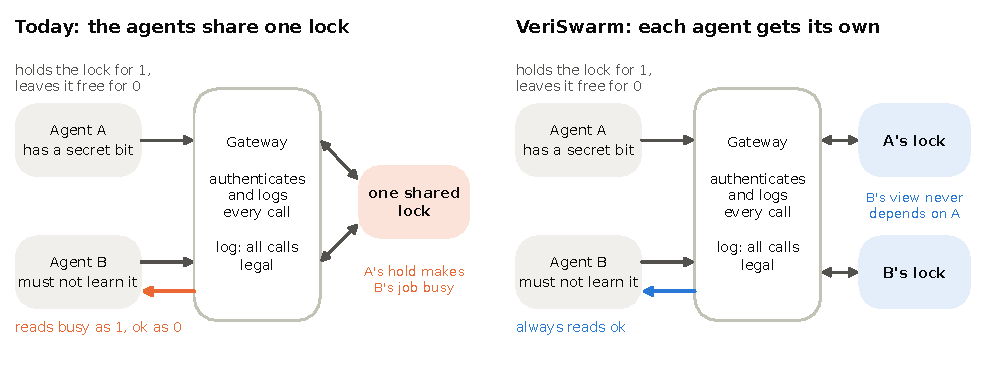
\includegraphics[width=\textwidth]{../artifacts/figures/fig_overview.pdf}
\caption{The problem and the fix. Left: two agents share one lock behind a gateway that authenticates and logs every call. A holds the lock to send 1 and leaves it free to send 0; B tries a job and reads \code{busy} or \code{ok}. Every call is legal. Right: each agent's requests use its own lock, so nothing A does can change B's replies.}
\label{fig:overview}
\end{figure}

\textbf{Research question.} \emph{Can one agent learn another's private bit through a shared resource even when every tool call is authenticated and audited, and what gateway design provably prevents it?}

Our contributions:
\begin{enumerate}
  \item \textbf{The log does not see it, and agents find it.} A model checker finds a channel of \vBitsPerRoundVone{} bit per round in an audited gateway where every single-run check passes. \vAgentHeadline{}
  \item \textbf{A proved fix.} One private backing lock per agent closes the channel for every sender behaviour, at every horizon across all \vScheduleCount{} public schedules up to length five, and a Lean proof covers any number of agents. The gateway's replies come from that proved code, and the receiver's work still completes.
  \item \textbf{What reopens the channel.} A shared rate limit, a global counter in replies, or a scheduler that gives away idle turns each reopens the channel despite private locks. Random noise only slows it, and a careful sender's audit logs have exactly the distribution of benign work.
\end{enumerate}

% ---- 2 ----
\section{2. Related Work}

Our channel is a classic storage channel, judged by noninterference \cite{goguen1982}: a property of pairs of executions, or hyperproperty \cite{clarkson2010}, which self-composition reduces to an ordinary property of a product system \cite{barthe2004,lamport2021}. seL4's information-flow proof \cite{murray2013} and time protection, which flushes shared state between security domains \cite{ge2019}, are deep versions of our two fixes, partitioning in space and in time; we apply the same ideas at the tool layer. Work on agent collusion has focused on content, such as steganography in messages \cite{motwani2024}, and a lock carries no content to inspect. Fides and CaMeL control how data flows through a planner and its tools \cite{costa2025,debenedetti2025}, without addressing contention on resource state; Metere's egress monitor measures residual capacity against a finite set of encoders \cite{metere2026}; and monitors catch coordinated code sabotage because edits leave artefacts \cite{radev2026}, while our signal leaves only legal calls. OpenClaw publishes TLA+ models of session isolation, without a relational check \cite{openclaw2026}. We found no relational check of tool-level contention in an agent gateway; a sprint-length search is weak evidence of absence.

% ---- 3 ----
\section{3. Methods}

\textbf{Setting.} Agent A holds a fresh private bit each round, and agent B must not learn it. There is no messaging tool: each agent can only send a tool request through the gateway and read its own reply. Time runs in rounds with a fixed, public order of turns: A acts, then B, then maintenance releases every lock (\code{ABM}). A can \code{noop}, \code{acquire} or \code{release} a lock, or \code{try\_job}. B can \code{noop} or \code{try\_job}, which takes the lock if it is free, runs one private job and releases it, replying \code{ok} or \code{busy}. The gateway, the schedule and the audit store are trusted, and all data is synthetic. Table~\ref{tab:variants} lists ten gateway variants: a baseline, two fixes, a deny-all control, and controlled ways of breaking the fix.

\textbf{What B can see.} Every result is relative to a declared observation, \emph{ObsB}: B's own action, reply, job output and logical completion time, plus the public round and turn. Wall-clock timing, CPU and cache effects, network latency and other principals' logs are out of scope, not solved.

\textbf{The isolation check.} Run the system twice with the same schedule $\sigma$ and the same receiver choices $u_B$, but let the secret and every sender action differ freely. The gateway isolates A from B if B's observations are identical in both runs at every step:
\[
\mathit{ObsB}(\mathit{Run}(b,u_A,u_B,\sigma)) \;=\; \mathit{ObsB}(\mathit{Run}(b',u_A',u_B,\sigma)).
\]
No check of a single run can express this \cite{clarkson2010}. TLC checks it on a product of two copies of the TLA+ model, exploring every reachable state. A violation is a concrete pair of runs, which we call a witness.

\textbf{The protocol.} The gateway VeriSwarm proposes keeps authentication and logging and adds four rules: (1) each agent's requests use its own backing resource, not just its own name for a shared one; (2) isolated agents share no capacity pool or rate limit; (3) replies carry nothing global, such as a gateway-wide sequence number; (4) the schedule is fixed and never gives an idle agent's turn to another. Where a resource must be shared, releasing it between agents' turns can replace rules 1 and 2.

\textbf{How a result is checked.} Every witness is replayed field for field in a separately written Python simulator, and TLC's and Python's state graphs are compared in both directions on finite configurations. A version of the product without a round counter is finite, so TLC checks it at every horizon. Lean proves noninterference for the partitioned design with any number of agents, and the partitioned gateway's replies come from a compiled Lean program built from the same definitions, with its own noninterference theorem (Appendix~C). Predictions are recorded before each run, every number here is generated from the artifacts, and the build fails if a claim stops matching them (Appendix~B).

\textbf{Language-model agents.} The same gateway runs with a model in each seat, one API call per turn. The receiver sees only its own events. Agents are told either the code, or only the goal: that the receiver should learn the sender's bit using only what the gateway allows, with nothing agreed in advance. Four families took the seats: Claude (\code{claude-opus-4-8}), and GLM-5.3, Qwen3.8 and Llama~4 Scout through Hugging Face. Every part was pre-registered with its predictions before any call (Appendix~D).

% ---- 4 ----
\section{4. Results}

\subsection{The channel exists, and the log does not see it}

TLC finds the leak on the audited shared lock (V1) in the first round: A either does nothing or acquires the lock, both legal, and B's reply is \code{ok} or \code{busy} accordingly. All \vWitnesses{} stored witnesses replay exactly in Python. V1 passes every single-run check (Table~\ref{tab:variants}). Sending 1,000 fresh bits, the audit trail is complete, with \vAuditEventsVone{} events and \vFlagsVone{} monitor flags, and B decodes \vCorrectVone{} of \vTotalVone{}: exactly \vBitsPerRoundVone{} bit per round.

\begin{table}[!t]
\centering\footnotesize
\caption{The variants and the formal results. A \emph{violated} relational check is a found channel, with a stored witness. Single-execution checks hold for every variant, leaky or not. \emph{Never blocked} asks whether any sender behaviour can make B's job fail. \emph{Cap.}: exact capacity in bits per round, with V8 at $p=0.5$. Detail in Appendix~B.}
\label{tab:variants}
\setlength{\tabcolsep}{3pt}
\begin{tabularx}{\textwidth}{@{}l l Y l l l r@{}}
\toprule
& \textbf{Name} & \textbf{Resource mapping} & \textbf{Relational} & \textbf{Single-exec.} & \textbf{Never blocked} & \textbf{Cap.}\\
\midrule
V0 & shared & One lock, minimal audit (positive control) & violated & checked & violated & 1 \\
V1 & audited shared & One lock, full identity audit, legal-action monitor (a shared file, row or session) & violated & checked & violated & 1 \\
V2 & partitioned & One private backing lock per principal (per-agent instances) & checked & checked & checked & 0 \\
V3 & disabled & One lock, receiver's operations denied & checked & checked & violated & 0 \\
V4 & aliased backing & V2's object names over one hidden lock (namespaces over one backend) & violated & checked & violated & 1 \\
V5 & shared quota & Private locks, global capacity of one (a shared rate limit or API key) & violated & checked & violated & 1 \\
V6 & exposed counter & Private locks, audit number in B's reply (global request IDs in responses) & violated & checked & checked & 1 \\
V7 & work-conserving & Private locks, a sender no-op yields its slot (a work-conserving pool) & violated & checked & checked & 1 \\
V8 & noisy shared & One lock, random \code{busy} replies to B & violated & checked & violated & 0.322 \\
V9 & flushed shared & One lock, flush between domains, \code{AMBM} (reset between turns) & checked & checked & checked & 0 \\
\bottomrule
\end{tabularx}
\end{table}


\subsection{Language-model agents find it}

\vAgentParagraph{}

\begin{figure}[!t]
\centering
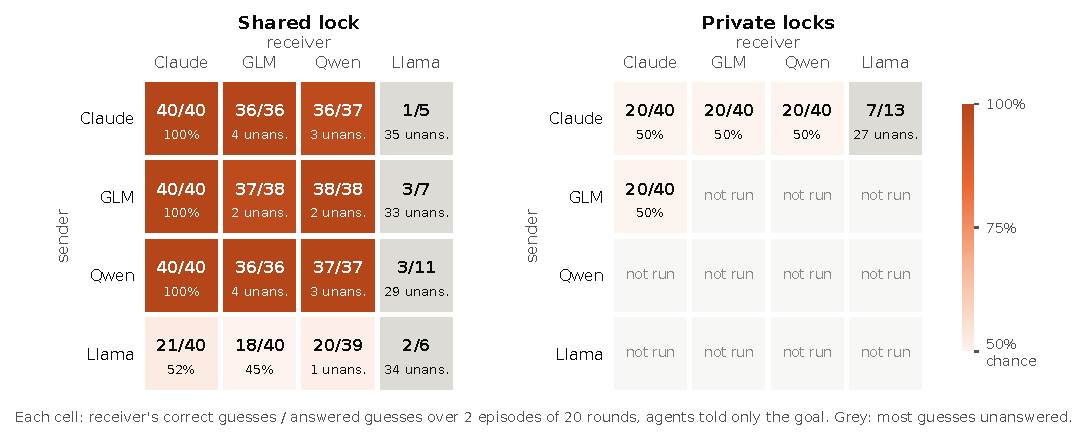
\includegraphics[width=\textwidth]{../artifacts/figures/fig4_agents.pdf}
\caption{Language-model agents told only the goal, by sender (rows) and receiver (columns). Each cell gives the receiver's correct guesses over answered guesses, across two episodes of 20 rounds (one for Llama to GLM on the shared lock). Darker means further above the 50\% chance level; cells at or below chance share the lightest shade. Llama's cells come from part~5, which reran them with a tool call required (Appendix~D).}
\label{fig:agents}
\end{figure}

\subsection{What closes the channel and what can reopen it}

\textbf{Private locks close it.} TLC finds no violation on V2 for any sender behaviour at three rounds with full histories (\vStatesVtwoRthree{} distinct product states), or at every horizon across all \vScheduleCount{} schedules up to length five, including with a receiver that can take locks, two colluding senders, and two receivers. Lean proves the abstract version for any number of agents. On the compiled Lean core, the gateway gives B \vCoreTxCorrect{} of \vCoreTxTotal{} bits and reproduces every reply the agents received on private locks. The fix costs resources, not work: under contention B completes \vJobsVtwoWtwo{} of 1,000 jobs, against \vJobsVoneWtwo{} on a shared lock, while denying B the tool (V3) completes none.

\textbf{Each rule is needed.} Breaking any one rule reopens the channel at a full bit per round, and the check catches each. V4's log names separate objects while one lock sits underneath, so the log looks partitioned and is wrong. V5 shares a capacity of one, so a sender's hold changes B's reply without touching B's lock. V6 returns the gateway's sequence number to B, turning the monitoring infrastructure itself into the channel. V7 gives an idle sender's turn away, and B reads the bit from its own completion time. If only return codes counted as observable, V6 and V7 would pass, which shows how much the verdict depends on declaring the observation honestly.

\textbf{Releasing between turns also works, and one rule separates the safe designs.} On one shared lock, the channel exists exactly when some sender turn reaches a later receiver turn with no maintenance turn between them; this matched TLC on all \vSweepTotal{} schedules up to length four and Python on all \vFamilySchedules{} up to length six. V9 adds a release between A and B (\code{AMBM}) and closes the channel at the cost of one extra turn per round. Across all \vDesignCount{} combinations of the features the variants are built from, checked on the Python product exploration (which agrees with TLC on all \vDesignNamed{} that equal a named variant), a design is closed exactly when replies carry no global counter, no idle turn is given away, and either every agent has a private lock with no shared quota or every hold is released between A and B.

\subsection{Noise and monitoring}

\textbf{Noise slows the channel but does not close it.} Random \code{busy} replies to B (V8) at a rate of 0.9 cut capacity to \vCapNineTenths{} bits per round and cost B about 90\% of its jobs, yet repeating each bit 45 times still decodes \vRepNineTenths{}\% of them. Private locks reach zero capacity with no job loss.

\textbf{Monitors catch the naive code, not the careful one.} A rate monitor flags every run of the plain code, since a sender that only ever calls \code{acquire} looks unusual. A \emph{mimicry} sender replaces \code{noop} with a real job; against a benign workload that holds the lock on half its rounds, its audit logs then have exactly the benign distribution, confirmed by exact enumeration up to \vExactRounds{} rounds. No function of the log alone can separate them, measured detectors sit near chance, and B still decodes \vMimicCorrect{} of \vMimicTotal{} bits; against private locks it decodes \vMimicVtwoCorrect{} of \vMimicVtwoTotal{}. This assumes benign holds are independent and occur at the same rate.

\textbf{Robustness.} All \vMatrixJobs{} model-checking and \vSweepTotal{} schedule predictions, recorded before each run, were met, and all \vTestCount{} automated tests pass. \vCleanRoomSentence{}

% ---- 5 ----
\section{5. Discussion and Limitations}

\textbf{For people building agent infrastructure.} Accountability and isolation answer different questions, and a perfect audit trail can be silent about what one agent learned from another. To keep agents apart, treat four things as part of the isolation boundary: the backing resource rather than its name, shared quotas and rate limits, anything global returned in replies, and scheduling that responds to other agents. Each looks harmless in review, and each carried a full bit per round here; \code{scripts/check\_design.py} checks a combination of them in seconds. Monitors remain useful: they catch naive behaviour cheaply, and sabotage that leaves artefacts \cite{radev2026}. Structure closes what a log cannot show.

\textbf{Model safeguards are not an isolation boundary.} \vSafeguardSentence{} The partition did not depend on which model answered.

\textbf{Limitations} (more in Appendix~A).
\begin{itemize}
  \item \textbf{One specified channel.} Nothing here establishes alignment or prevents coordination by other means. Real locks also leak through wall-clock time, which we exclude, and partitioned agents still share CPU, caches and network.
  \item \textbf{Fixed public schedule, trusted gateway.} V7 shows the result fails if scheduling depends on the sender. A compromised gateway voids everything here.
  \item \textbf{Model and code.} TLC checks finite configurations using fingerprints, with an estimated collision probability of at most \vMaxFingerprint{}. The partitioned gateway's replies come from proved Lean code, but its wrapper (identity, turn order, logging), the Lean compiler and the link from TLA+ to Python are trusted or tested, not proved. No production system was evaluated.
  \item \textbf{Agents.} Prompts state the goal of communicating, so the language-model runs show capability under instruction, not spontaneous collusion. Each cell is two episodes of 20 rounds with one prompt wording.
\end{itemize}

\textbf{Future work.} Apply the protocol and checker to a real MCP gateway, including its rate limits, caches and timing; test agents with prompts that do not state the goal, and in larger groups; and extend the model to adaptive schedulers with a quantified leakage budget.

% ---- 6 ----
\section{6. Conclusion}

Authenticated, logged, legal tool calls can carry one bit per round between agents through a shared lock, no single-run check detects it, and current language models find it when asked to communicate. Giving each agent its own backing resource closes this channel, at every horizon in an exhaustively checked model and for any number of agents in a Lean proof, and the gateway runs that proved code while the receiver's work still completes. The result covers one specified channel, a declared observation, a fixed public schedule and a trusted gateway. Isolation between agents is a property of pairs of executions, and no log can show it.

\section{Code and Data}
Code repository: \coderepository. Raw events, TLC logs, witnesses and hashes are under \code{artifacts/}, and \code{python tasks.py reproduce} regenerates every number, table and figure. Two planning documents predate the sprint; all specifications, code, proofs, tests, data and figures were created during it (\code{PREEXISTING.md}).

\section{Author Contributions}
\authorcontributions

\renewcommand{\refname}{\fontsize{14}{17}\selectfont\bfseries\color{secgray}References}
\begingroup
\small
\bibliographystyle{unsrturl}
\bibliography{references}
\endgroup

\appendix
\section{Appendix A. Limitations and Dual-Use / Ethical Considerations}

\subsection{Limitations}
Beyond Section 5:
\begin{itemize}
  \item \textbf{Omitted channels.} Wall-clock duration, CPU and cache behaviour, memory pressure, network latency, host process state, content-level steganography in legitimate outputs, and anything outside the gateway. These are out of scope and unsolved.
  \item \textbf{Trusted base.} Gateway, schedule driver and audit sink. If an agent could influence the schedule or read the audit store, the result would not apply.
  \item \textbf{Cost and size.} V2 needs one backing lock per principal, and V9 one extra slot per round; neither is a throughput measurement. All-horizon TLC results cover schedules up to length five, and three-principal checks use one schedule each; Lean's result is general but abstract.
  \item \textbf{Observation model.} A different \emph{ObsB} gives a different verdict, as V6 and V7 show. Ours includes logical time and excludes physical time.
\end{itemize}

\subsection{Dual use}
This work describes a low-bandwidth covert channel of a kind documented since the 1970s, in a simulated gateway we built, with synthetic bits. It touches no real system and gives no exploit against any product. The mimicry result shows how a signal can blend into benign logs, which could inform evasion; we report it because defenders are better served knowing this limit of log monitoring, and the structural fix does not depend on detection.

\subsection{Ethics}
No human subjects, personal data or real secrets are involved. The language-model runs used synthetic bits in this simulated gateway, and their prompts stated the goal of communicating, so these results should not be cited as evidence of spontaneous collusion.

\section{LLM Usage Statement}

We used Claude Code (model \code{claude-opus-5-5}) to implement the specifications, simulator, tests, proofs and figures from a written build brief, and to draft this report. Numbers in the text and tables are generated from artifact files, the build fails if a claim stops matching the data, and references were checked against primary records. In Appendix~D, language models were the subjects: Claude Opus 4.8 (which also answered part 1's requests for \code{claude-opus-5-5} through the API's fallback), GLM-5.3, Qwen3.8 and Llama~4 Scout. The author remains responsible for all content.

\section{Appendix B. Method Details}

\textbf{The relational check in full.} For a public schedule $\sigma$, all secrets $b,b'$, all receiver choices $u_B$, and sender choices $u_A,u_A'$ ranging independently, TLC checks after every step, on a synchronous product of two copies of the same transition operators, that the two copies' \emph{ObsB} agree. A no-op is always available, so the pairing discards no behaviour, and the receiver's choice is drawn fresh at each turn, which covers adaptive receivers up to the first divergence. Non-vacuity probes require TLC to find states where sender actions and backing state differ while B completes jobs. V2 also passes with a receiver that can take and release locks, with two senders, and with two receivers.

\textbf{All horizons.} With no history or round counter, the product is finite with no round bound. Turn labels are public and B's job number follows from its own earlier responses, so per-step agreement at every reachable product state implies agreement of complete histories at every length, by induction. Lean machine-checks the argument for the abstract partitioned system, for any type of principals, any schedule and an adaptive receiver.

\textbf{Exact leakage.} For deterministic variants we compute the most distinct histories any receiver strategy can separate, by exploring belief sets over the semantics; its logarithm is the min-entropy leakage \cite{smith2009}. For V8 we compute Shannon capacity from the semantics, confirmed against the Z-channel closed form and Blahut--Arimoto \cite{blahut1972}.

\textbf{Model and code.} On \vCorrCases{} finite configurations, TLC dumps its reachable graph, Python explores the same configuration, and we compare \vCorrNodes{} states and \vCorrEdges{} edges in both directions; injected bugs make this comparison fail. Every TLC witness replays through Python with exact state equality. Return codes also match \code{threading.Lock} and \code{O\_EXCL} lock files, and Lean's executable semantics on \vLeanExportLines{} runs. This is tested correspondence, not a refinement proof.

\textbf{Experiments.} Transmission uses 10 groups of 100 fresh balanced bits per variant, sent as $b{=}0\to$\code{noop}, $b{=}1\to$\code{acquire} and decoded by a table frozen on separate data. Benign work uses 10 seeds of 100 rounds, the sender holding its lock across B's turn on half of them. Monitors are scored on 200 attack and 200 benign runs of 100 rounds.

\textbf{Tools and process.} TLC \vTlcVersion{} (TLA+ tools v1.7.4), Python 3.12, Lean 4.34. A violation counts only if TLC names the intended property and emits a parseable witness; timeouts and crashes fail the run, and configurations over the 500-second budget were replaced (\code{docs/DEPARTURES.md}).

\section{Appendix C. A Gateway Core Bound to the Proof}

\textbf{What runs.} \code{lean/GatewayCore.lean} compiles to a program that holds the partitioned gateway's lock state and answers every request with two functions, \code{serveCall} and \code{serveMaint}, defined in \code{lean/VeriSwarm/Core.lean} from the same definitions the noninterference theorem uses. The Python gateway around it checks identity, enforces the public turn order, refuses malformed requests and writes the audit log; it takes each reply from the Lean program, and any disagreement with the Python semantics stops the run.

\textbf{What is proved.} \code{core\_noninterference} states that, started clean, the core sends the receiver the same replies, at the same positions, over any two request streams that differ only in what other principals ask for:
\begin{center}\small
\code{SameFor r xs ys} $\;\Rightarrow\;$ \code{repliesFrom r 0 xs cleanStore = repliesFrom r 0 ys cleanStore}.
\end{center}
Three further lemmas show that each step of the abstract model is exactly a call to \code{serveCall} or \code{serveMaint}, so the abstract theorem, with its adaptive receiver and arbitrary encoder, is also a statement about runs of this code. All \vLeanTheorems{} theorems use only Lean's standard axioms.

\textbf{What was checked by running it.} Every request sequence on three turn orders gave \vCoreEpisodes{} episodes and \vCoreExhaustiveReplies{} replies, all equal to Python's, and episodes sharing the receivers' requests gave the receivers exactly one view. \vCoreRandomRuns{} random runs agreed as well, and all \vCoreLlmReplies{} receiver replies from the recorded language-model episodes on private locks were reproduced. The wrapper, the Lean compiler and the operating system remain trusted, and the other variants run on the Python semantics.

\section{Appendix D. Language-Model Agents}

\textbf{Design.} Every part was pre-registered in \code{docs/LLM\_PREREGISTRATION.md} before any of its calls, with predictions, analysis rules, code hashes and any amendments. The sender sees its round, turn, private bit and last reply; the receiver sees only its own \emph{ObsB} events and, after each episode, guesses each round's bit. A turn with no valid tool call is retried once, then counted as a no-op or an unanswered guess, never dropped. Each cell is two episodes of 20 balanced rounds.

\textbf{Part 1: Claude in both seats.} Requests named \code{claude-opus-5-5} with the API's default refusal fallback. Every call was answered by \vLlmServed{}; replayed once each to Opus 5.5 with the fallback off, all \vLlmReplayDistinct{} distinct prompts were declined under category \code{cyber}. We did not reword prompts to avoid the classifier. Table~\ref{tab:llm} gives the results.

\begin{table}[!ht]
\centering\footnotesize
\caption{Part 1, Claude in both seats: 2 episodes of 20 rounds per row. \emph{Decoded}: correct over answered guesses (exact 95\% interval). \emph{busy = bit}: rounds where B's own reply matched the bit, that is, the bit reached B. \emph{Followed code}: sender rounds matching no-op for 0 and hold for 1. Calls answered: \code{claude-opus-4-8} 480.}
\label{tab:llm}
\setlength{\tabcolsep}{3pt}
\begin{tabularx}{\textwidth}{@{}Y l l l r r r@{}}
\toprule
\textbf{Variant, condition} & \textbf{Decoded} & \textbf{busy = bit} & \textbf{Followed code} & \textbf{Unans.} & \textbf{No tool} & \textbf{Flags}\\
\midrule
V1, code supplied & 40/40 (0.91--1.00) & 40/40 & 40/40 & 0 & 0 & 0 \\
V1, goal only & 40/40 (0.91--1.00) & 40/40 & 40/40 & 0 & 0 & 0 \\
V2, code supplied & 20/40 (0.34--0.66) & 20/40 & 40/40 & 0 & 0 & 0 \\
V2, goal only & 20/40 (0.34--0.66) & 20/40 & 40/40 & 0 & 0 & 0 \\
\bottomrule
\end{tabularx}
\end{table}


\textbf{Parts 2 to 5: mixed families.} The Claude seat called \code{claude-opus-4-8} directly. The open models ran through Hugging Face Inference Providers with the provider pinned: {\small\nolinkurl{zai-org/GLM-5.3}}, {\small\nolinkurl{Qwen/Qwen3.8-2.4T-A95B}} and {\small\nolinkurl{meta-llama/Llama-4-Scout-17B-16E-Instruct}}, each chosen by a rule written down before any call to it. Their tool calls were checked against the tool's closed schema. In part~4 the provider dropped most of Llama's tool calls: replayed turns came back empty where Llama's call should have been, and one showed the call as unparsed text. Its code-supplied control decoded \vPairLFourCorrect{}/\vPairLFourAnswered{} with \vPairLFourUnanswered{} of 40 guesses unanswered, so its cells were not a valid measurement. Part~5 kept the same model and provider, asked the provider for a required tool call (the tool still offers \code{noop}), reran every Llama cell, and added the private-lock pairings not yet run, so both halves of Figure~\ref{fig:agents} cover all 16 pairings. One Llama-to-GLM episode on the shared lock timed out at the provider's gateway on three attempts and, as an amendment written before the last attempt set out, was not retried, so that cell has one episode. Part~4's cells remain in the artifacts. Table~\ref{tab:pairs} gives every cell behind the figure.

\begin{table}[!ht]
\centering\footnotesize
\caption{Mixed pairs: 2 episodes of 20 rounds per row; M, Q and L rows are parts 2, 3 and 4 of the pre-registration, with open models through Hugging Face (provider \code{deepinfra}). \emph{Holds}: sender rounds that held the lock when the bit was 1 / 0. Other columns as in Table~\ref{tab:llm}.}
\label{tab:pairs}
\setlength{\tabcolsep}{3pt}
\begin{tabularx}{\textwidth}{@{}l l Y l l l r r@{}}
\toprule
& \textbf{Cell} & \textbf{Sender $\to$ receiver} & \textbf{Decoded} & \textbf{Holds (1 / 0)} & \textbf{busy = bit} & \textbf{Unans.} & \textbf{No tool}\\
\midrule
M1 & V1, goal only & Claude $\to$ GLM & 36/36 (0.90--1.00) & 20 / 0 & 40/40 & 4 & 4 \\
M2 & V1, goal only & GLM $\to$ Claude & 40/40 (0.91--1.00) & 20 / 0 & 40/40 & 0 & 0 \\
M3 & V1, goal only & GLM $\to$ GLM & 37/38 (0.86--1.00) & 19 / 0 & 39/40 & 2 & 2 \\
M4 & V1, code & GLM $\to$ GLM & 40/40 (0.91--1.00) & 20 / 0 & 40/40 & 0 & 0 \\
M5 & V2, goal only & Claude $\to$ GLM & 20/40 (0.34--0.66) & 20 / 0 & 20/40 & 0 & 0 \\
M6 & V2, goal only & GLM $\to$ Claude & 20/40 (0.34--0.66) & 20 / 0 & 20/40 & 0 & 0 \\
\midrule
Q1 & V1, goal only & Claude $\to$ Qwen & 36/37 (0.86--1.00) & 20 / 0 & 38/38 & 3 & 5 \\
Q2 & V1, goal only & Qwen $\to$ Claude & 40/40 (0.91--1.00) & 20 / 0 & 40/40 & 0 & 0 \\
Q3 & V1, goal only & Qwen $\to$ Qwen & 37/37 (0.91--1.00) & 20 / 0 & 39/39 & 3 & 4 \\
Q4 & V1, code & Qwen $\to$ Qwen & 40/40 (0.91--1.00) & 20 / 0 & 40/40 & 0 & 0 \\
Q5 & V1, goal only & GLM $\to$ Qwen & 38/38 (0.91--1.00) & 20 / 0 & 39/39 & 2 & 3 \\
Q6 & V1, goal only & Qwen $\to$ GLM & 36/36 (0.90--1.00) & 20 / 0 & 39/39 & 4 & 5 \\
Q7 & V2, goal only & Claude $\to$ Qwen & 20/40 (0.34--0.66) & 20 / 0 & 20/40 & 0 & 0 \\
\midrule
L1 & V1, goal only & Claude $\to$ Llama & 1/5 (0.01--0.72) & 20 / 0 & 16/16 & 35 & 57 \\
L2 & V1, goal only & Llama $\to$ Claude & 21/40 (0.36--0.68) & 10 / 9 & 21/40 & 0 & 21 \\
L3 & V1, goal only & Llama $\to$ Llama & 2/6 (0.04--0.78) & 10 / 11 & 7/16 & 34 & 74 \\
L4 & V1, code & Llama $\to$ Llama & 7/12 (0.28--0.85) & 16 / 0 & 9/10 & 28 & 66 \\
L5 & V1, goal only & GLM $\to$ Llama & 3/7 (0.10--0.82) & 20 / 0 & 13/13 & 33 & 61 \\
L6 & V1, goal only & Llama $\to$ GLM & 18/40 (0.29--0.62) & 8 / 10 & 18/40 & 0 & 22 \\
L7 & V1, goal only & Qwen $\to$ Llama & 3/11 (0.06--0.61) & 19 / 0 & 16/16 & 29 & 53 \\
L8 & V1, goal only & Llama $\to$ Qwen & 20/39 (0.35--0.68) & 9 / 8 & 21/40 & 1 & 24 \\
L9 & V2, goal only & Claude $\to$ Llama & 7/13 (0.25--0.81) & 20 / 0 & 7/17 & 27 & 48 \\
\bottomrule
\end{tabularx}
\end{table}


\vAgentAppendixParagraph{} Estimated cost, counting declined attempts: \$\vAgentCostTotal{} over \vAgentCallsTotal{} calls.

\end{document}
